\documentclass{beamer}

\usetheme{uhh}
\showtotalframenumber
\showuhhlogoeachframe
\showsections

\usepackage{amsmath}
\usepackage{graphicx}
\usepackage{color}
\DeclareMathOperator*{\argmin}{arg\,min}

\usepackage{listings}
\lstset{
  language=python
  }

\title{Deep Learning for Language and Speech}
\subtitle{Tensorflow tutorial based on slides by Fabian Barteld and Benjamin Milde}
\author{Prof. Dr. Chris Biemann, \underline{Benjamin Milde}}
\date[18.10.2018]{Oct 18, 2018}

\AtBeginSection[]
{
   %%%%% section title
   % This is how it would look like in Beamer:
   % \begin{frame}
   %     \frametitle{Overview}
   %     \tableofcontents[sections={2-3},currentsection,sectionstyle=show/hide,subsectionstyle=hide]
   % \end{frame}
  \begin{frame}[plain]
  \begin{tikzpicture}[overlay]
    \relax%
    \fill[blueuhh,opacity=1] (-10,-10)
    rectangle(\the\paperwidth,\the\paperheight);
  \end{tikzpicture}
   \begin{tikzpicture}[overlay]
    \relax%
    \fill[white,opacity=1] (-5,-1.2)
    rectangle(\the\paperwidth,0.5) node[pos=0.5,black]{\LARGE\insertsectionhead};
  \end{tikzpicture}
  \end{frame}

  %%%% add subsection to show navigation dots
  \subsection{}
}

\begin{document}

\maketitle

%\begin{frame}
%  \frametitle{Overview}
%
%  \begin{itemize}
%		\item Tensorflow Introduction / First session
%		\item Regression models
%		\item Neural tagger (DNN)
%		\item Implementing Word2Vec	
%		\item \textcolor{greyuhh}{Introduction to Tensorboard}
%		\item\textcolor{greyuhh}{Neural tagger (LSTM)}
%		\item \textcolor{greyuhh}{RNN language model (LSTM)}
%		\item \textcolor{greyuhh}{Maybe: Convolutions}
%	\end{itemize}
%\end{frame}

\section{Introduction}

\begin{frame}
\frametitle{Structure of the seminar}
  \begin{itemize}
    \item Welcome to the seminar "Deep Learning for Language and Speech"!
  	\item Introduction tutorial, teaching you Tensorflow and how to train your neural network models, hands on, 5-6 sessions (now)
  	\item Working in teams on training deep neural networks for NLP or speech problems, starting December
  	 \item At the end of the seminar: present your work, hand in small report (max. 8 pages)
  \end{itemize}
\end{frame}

\begin{frame}
\frametitle{Structure of the seminar}
  \begin{itemize}
	\item Before we continue:
  	\item E-mail: milde@informatik.uni-hamburg.de, please send me an e-mail with the title "DL Seminar"
  	\item Also, slides will be available here: \url{http://ltdata1.informatik.uni-hamburg.de/lt_deeplearning_seminar_WS1819/} \\ (User: student Password: dl\_seminar\_1718)
  \end{itemize}
\end{frame}

\begin{frame}
\frametitle{Structure of the seminar}
  \begin{itemize}
  	\item Who knows Python/numpy? There will be additional reading material if you're new to the language
  	\item Tutorial is hands on - \textbf{you need to bring your laptop}
  	\item Easiest installation of all required software is under Linux, e.g. Ubuntu
  	\item But Windows/Max OS X is also possible
  \end{itemize}
\end{frame}

\begin{frame}
\frametitle{Introduction}
  \begin{itemize}
	\item TensorFlow started as DistBelief at Google Brain in 2011
	\item Publicly released as  open source software on November 9, 2015
	\item Written in C++, Python bindings for rapid prototyping (best documented interface)
	\item Other bindings exist: Java, Scala, C\sharp , Rust, Go, Haskell, JavaScript, ...
    \item Similar projects exist: e.g. Theano, PyTorch, Dynet. All share the idea of using computation graphs.
  \end{itemize}
\end{frame}

\begin{frame}
  \frametitle{Main concepts}
  \begin{itemize}
		\item TensorFlow computations are expressed as stateful dataflow graphs
		\item Graphs contain operations (ops) on Tensors
		\item In TensorFlow lingu, a tensor is any n-d array. A scalar is a tensor
      of rank 0, a vector of rank 1, a matrix of rank 2.
		\item A Tensorflow rank is not the same as a matrix rank!
		\item The shape of a tensor with rank 2 is a tuple of dimensions, e.g. (128, 256) is a 128 x 256 matrix. 
		\item Tensors of rank 3 are heavily used in feed forward networks, an example is a tensor with shape (128, 128, 256) 
  \end{itemize}
\end{frame}

\begin{frame}[fragile]
  \frametitle{Layer based APIs vs. Graphs based}
  
A typical  layer API (not TensorFlow code):
  
  \begin{lstlisting}
model.add(Conv2D(64, (3, 3), activation='relu'))
model.add(MaxPooling2D(pool_size=(2, 2)))
model.add(Dropout(0.25))
model.add(Flatten())
model.add(Dense(128, activation='relu'))
model.add(Dropout(0.5))
model.add(Dense(num_classes, activation='softmax'))
\end{lstlisting}

This is fine (and very readable!) for models that can be described by stacking individual layers
  
\end{frame} 

\begin{frame}[fragile]
  \frametitle{Layer based APIs vs. Graphs based}
  
Disadvantage: Difficult to express structures like these:
  
    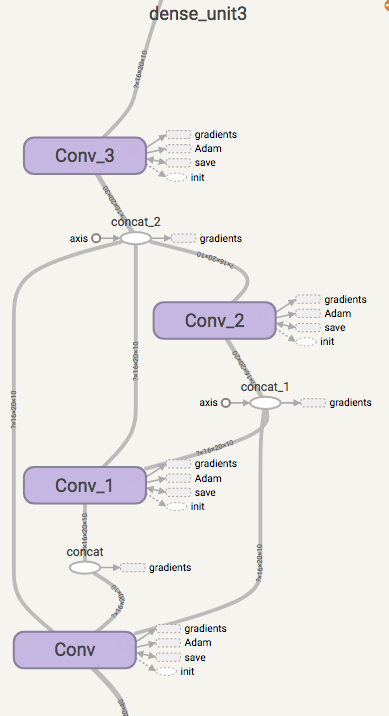
\includegraphics[angle=-90,width=0.75\textwidth]{graph_example}

Increasing evidence that these kind of deeply connected networks are very useful.
  
\end{frame} 

\begin{frame}[fragile]
  \frametitle{Layer based APIs vs. Graphs based}
  \begin{itemize}
		\item  Since Tensorflow uses computation graphs, the declaration of the model allows for a higher expressivity
		\item  Has a steeper learning curve in the beginning
		\item  In the newer versions of Tensorflow, you can also mix layer-like APIs (e.g. TF-Slim, Keras) with the computation graph
		\item  We will focus on not using any short cuts, as this has a higher learning effect and we will only make use of standard Tensorlfow ops in the beginning
  \end{itemize}
\end{frame} 

\begin{frame}
\frametitle{First steps - Install required software }

\begin{itemize}
	\item Detailed installation instructions: \url{http://ltdata1.informatik.uni-hamburg.de/lt_deeplearning_seminar_WS1819/}
	\item TL;DR basic installation with Linux: pip3 install --upgrade numpy matplotlib scipy pyqt5 tensorflow
	\item (If you have a CUDA-enabled Nvidia GPU in your laptop, install tensorflow-gpu instead of the tensorflow package)
	\item For Mac Os X: install python3 and pip3 with brew (see http://brew.sh)
	\item For Windows: install Anaconda
\end{itemize}

\end{frame} 

\begin{frame}[fragile]
\frametitle{First steps - Lets open spyder}

type spyder3 in the console:

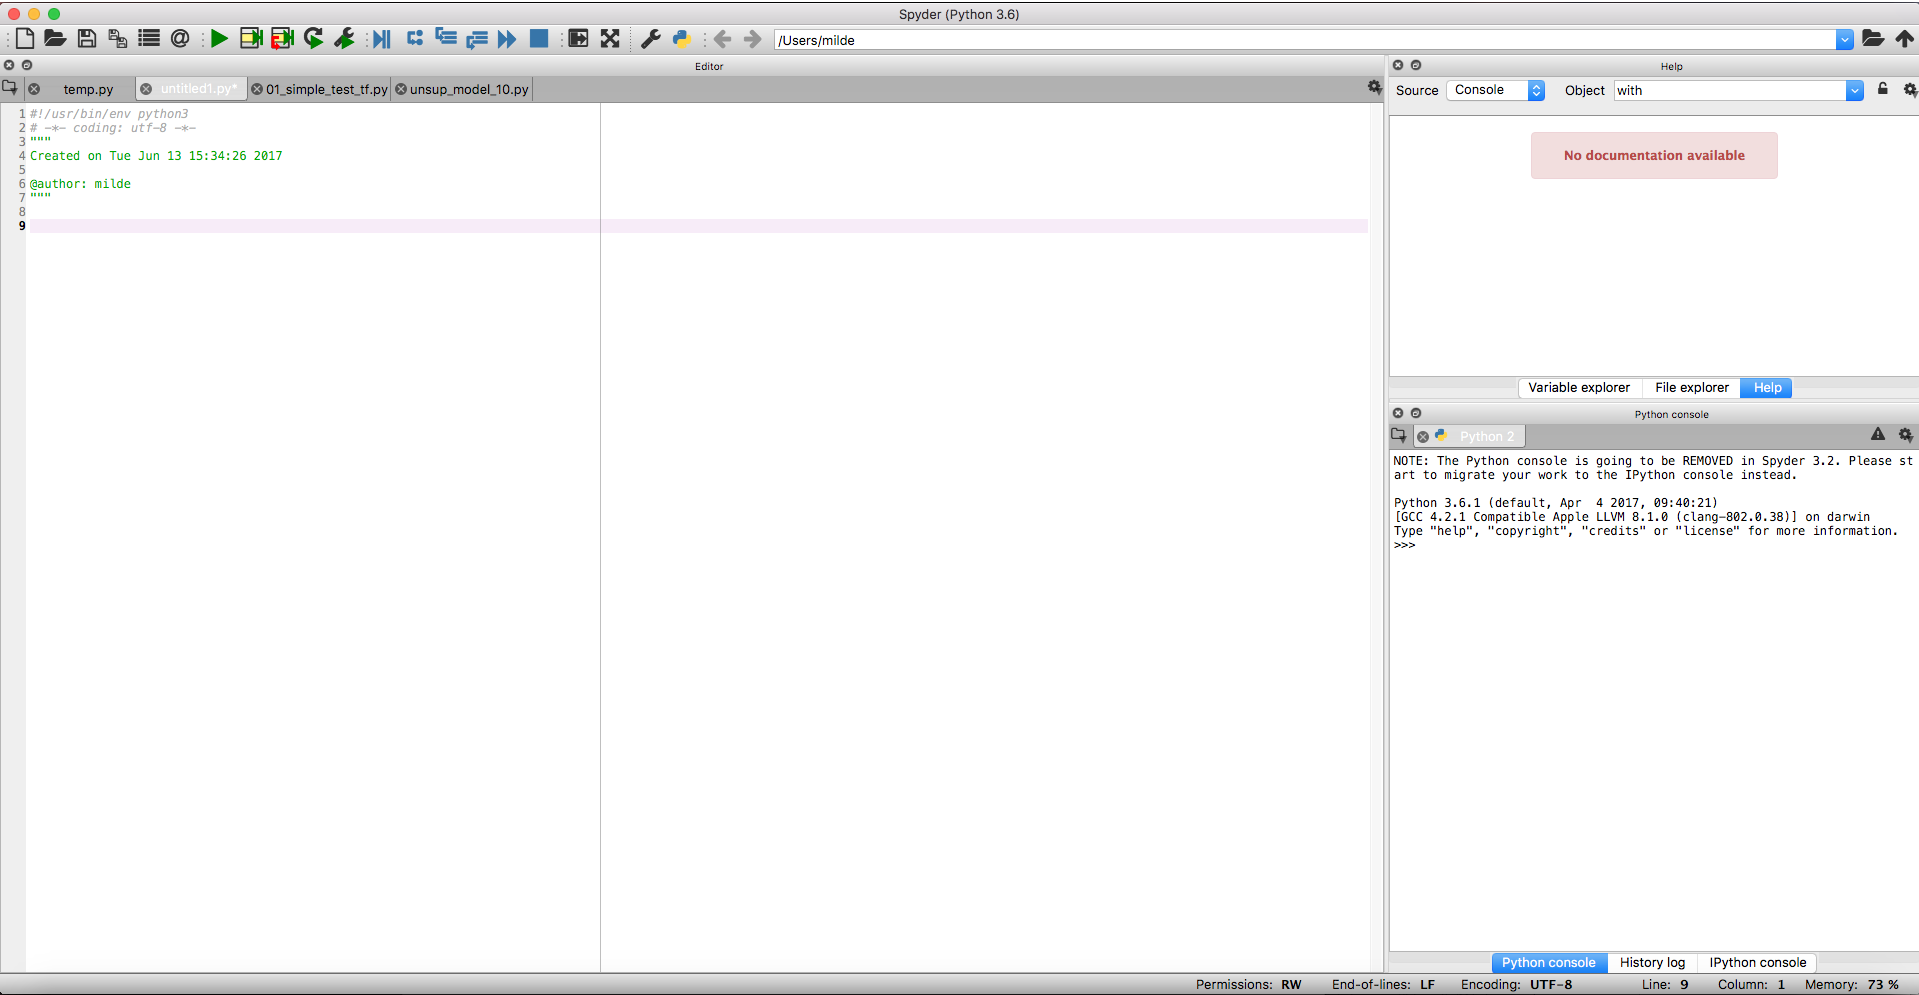
\includegraphics[width=0.95\textwidth]{spyder}

\end{frame} 

\begin{frame}[fragile]
\frametitle{First steps - Necessary imports}

\begin{lstlisting}
import numpy as np
import tensorflow as tf
\end{lstlisting}

\begin{itemize}
 	\item Outside of graph computations, we usually store data in Numpy arrays.
 	\item Numpy arrays are the main objects to transfer data to inputs of the graph and from outputs of the graph.
 	\item Numpy arrays are also an abstraction for (homogeneous) multidimensional arrays.
\end{itemize}

\end{frame} 

\begin{frame}[fragile]
\frametitle{Generating some random data}

\begin{lstlisting}
#some random test data
a_data = np.random.rand(256)
b_data = np.random.rand(256)
\end{lstlisting}

\begin{itemize}
	\item Now a and b contain vectors of length 256 with random floats. E.g. print(a\_data) returns:
\end{itemize}

\begin{lstlisting}
[ 0.54976368  0.87790201  0.96528541 ..., 
 0.05281365  0.48556404  0.46848266]
  \end{lstlisting}

\end{frame} 


\begin{frame}[fragile]
\frametitle{Declare the computation graph}

\begin{lstlisting}
#construct the graph
a = tf.placeholder(tf.float32, [256])
b = tf.placeholder(tf.float32, [256])

x = a+b 
\end{lstlisting}

\begin{itemize}
\item The placeholders can later be used to input data to the computation graph
\item The operation x = a+b does not immediately add something, it creates a graph.
\item In fact, print(x) returns: 
\end{itemize}

\begin{lstlisting}
Tensor("add:0", shape=(256,), dtype=float32)
\end{lstlisting}

\end{frame} 

\begin{frame}[fragile]
\frametitle{A session on a computation device}

\begin{lstlisting}
with tf.device('/cpu'):
    with tf.Session() as sess:
       x_data = sess.run(x, {a: a_data, b: b_data})  
       print(x_data)
\end{lstlisting}

\begin{itemize}
\item This fills the inputs a and b with a\_data and b\_data (our random data), runs the computation graph and retrieves the results of x in x\_data
\item Obviously not terrible useful as is, but you could run the operation easily on a gpu by changing tf.device('/cpu') to  tf.device('/gpu:1'). Copying data to and from the GPU is handled automatically for you.
\end{itemize}

\end{frame} 

\begin{frame}[fragile]
\frametitle{Small warm up exercise!}

\begin{itemize}
	\item Calculate the matrix multiplication of a and b. We also change a and b to random matrices:
\end{itemize}

\begin{lstlisting}
a = np.random.rand(256, 128)
b = np.random.rand(128, 512)
\end{lstlisting}

\begin{itemize}
	\item Calculate the resulting matrix of shape (256, 512) in TensorFlow.
\end{itemize}

\end{frame} 

%\section{Simple Optimization}
%
%% https://medium.com/@saxenarohan97/intro-to-tensorflow-solving-a-simple-regression-problem-e87b42fd4845
%% https://github.com/aymericdamien/TensorFlow-Examples/blob/master/examples/2_BasicModels/linear_regression.py
%\begin{frame}
%  \frametitle{Linear Regression}
%
%  \begin{itemize}
%  \item Given: $(x_1, y_1)$, \ldots, $(x_n,y_n)$
%  \item Goal: find $w$ and $b$ such that:
%    \begin{displaymath}
%      \argmin_{w, b} \frac{\sum^n_{i=1} (\hat{y}_i - y_i)^2}{n}
%    \end{displaymath}
%    where $\hat{y}_i = wx_i + b$.
%  \end{itemize}
%
%\end{frame}
%
%\begin{frame}[fragile]
%  \frametitle{Define model parameters}
%  Model: $\hat{y}_i = wx_i + b$
%
%\begin{lstlisting}
%w = tf.Variable(np.random.randn(), name="weight")
%b = tf.Variable(np.random.randn(), name="bias")
%\end{lstlisting}
%\end{frame}
%
%\begin{frame}[fragile]
%  \frametitle{Define the model}
%
%  \begin{displaymath}
%    \begin{pmatrix} \hat{y}_1\\\vdots\\\hat{y}_n\end{pmatrix} =
%    \begin{pmatrix} w\\\vdots\\w\end{pmatrix} *
%    \begin{pmatrix} \hat{x}_1\\\vdots\\\hat{x}_n\end{pmatrix} +
%    \begin{pmatrix} b\\\vdots\\b\end{pmatrix}
%  \end{displaymath}
%
%\begin{lstlisting}
%yhat = tf.add(tf.multiply(X, w), b)
%\end{lstlisting}
%
%{\footnotesize The scalars $w$ and $b$ are converted into vectors of the same
%  length as X (broadcast); \url{https://www.tensorflow.org/performance/xla/broadcasting}}
%
%\end{frame}
%
%\begin{frame}[fragile]
%  \frametitle{Define the loss}
%
%\begin{lstlisting}
%loss = tf.reduce_mean(tf.square(y - yhat))
%\end{lstlisting}
%
%\end{frame}
%
%
%\begin{frame}[fragile]
%  \frametitle{Optimization}
%
%\begin{lstlisting}
%epochs = 10
%optimizer = tf.train.GradientDescentOptimizer(
%    learning_rate).minimize(loss)
%
%with tf.Session() as sess:
%    ## initalize parameters
%    sess.run(tf.global_variables_initializer())
%
%    for i in list(range(epochs)):
%        ## run one epoch
%        sess.run(optimizer)
%        ## print result and loss
%        print(sess.run(yhat) + ' ' + sess.run(loss))
%\end{lstlisting}
%
%\end{frame}
%
%\begin{frame}[fragile]
%  \frametitle{Hands on: Simple optimization}
%
%  \begin{enumerate}
%  \item Do a linear regression to learn $y = 2x + 1$
%  \item Do a multiple linear regression with Boston housing prices
%  \end{enumerate}
%
%\begin{lstlisting}
%from sklearn.datasets import load_boston
%from sklearn.preprocessing import scale
%
%total_X, total_Y = load_boston(True)
%total_x = scale(total_x)
%\end{lstlisting}
%\end{frame}
%
%% https://www.tensorflow.org/tutorials/wide
%% https://github.com/aymericdamien/TensorFlow-Examples/blob/master/examples/2_BasicModels/logistic_regression.py
%\begin{frame}
%  \frametitle{Logistic regression}
%
%  TODO
%  tf.sigmoid
%
%\end{frame}
%
%\begin{frame}
%  \frametitle{Hands on: Regression model}
%
%  TODO: more complex example
%\end{frame}

\end{document}


%%% Local Variables:
%%% mode: latex
%%% TeX-engine: luatex
%%% End:
